% Contenidos del capítulo.
% Las secciones presentadas son orientativas y no representan
% necesariamente la organización que debe tener este capítulo.
\section{Análisis}
En esta sección se va a analizar los casos de uso necesarios para la implementación de
nuestra aplicación, relacionándolos con los requisitos deducidos en el apartado anterior.
Además, también se va a definir los actores que interactúan con el sistema y un primer
modelo de datos que seguirá la aplicación.

\subsection{Diagrama de casos de uso} \label{sec:casosuso}

En la Figura~\ref{fig:casos} se observan todos los casos de uso identificados con respecto a la toma de requisitos realizada. En este caso se han identificado los siguientes actores, detallándolos de menos a más privilegios dentro de la aplicación web como se aprecia en la Figura~\ref{fig:casos_usuario} que incluye un diagrama de clases de herencia de actores funcionales en la plataforma web.
\begin{itemize}
    \item \textbf{Usuario:} Este actor es un usuario que accede a la aplicación web sin registrarse, podrá realizar solo labores de consulta de información sobre la aplicación.
    \item \textbf{Usuario registrado:} Este actor se identificara cuando el el actor usuario se haya registrado o haya iniciado sesión correctamente y podrá realizar las acciones necesarias para reservar la casa rural.
    \item \textbf{Cliente:} Este actor será un actor de tipo Cliente al que se le haya asignado una reserva y esta haya finalizado, lo que le dará derecho a dejar una reseña del alojamiento.
    \item \textbf{Gestor:} Este actor podrá realizar las acciones de aprobación y denegación de reservas realizadas por los clientes.
    \item \textbf{Sistema:} Este es un actor de tipo no funcional que realizara todas las labores del sistema, como son el refresco de los datos, el envío de correos de reserva y la extracción y actualización periódica de entidades externas.
\end{itemize}

\begin{figure}[h!tb]
    \centering
    
    \includegraphics[width=1\textwidth]{figs/casos2.png}
    \caption{Diagrama general de casos de uso.\label{fig:casos}}
    
\end{figure}

\begin{figure}[h!tb]
    \centering
    
    \includegraphics[width=0.5\textwidth]{figs/casos_usuario.png}
    \caption{Diagrama de los actores que interactuan en el sistema.\label{fig:casos_usuario}}
    

\end{figure}

A continuación, se van a definir cada uno de los casos de uso ilustrados en la Figura~\ref{fig:casos} y los requisitos con los que están involucrados.
Inicialmente, el usuario puede acceder al sistema de forma anónima, registrarse o iniciar sesión. 
En la Tabla~\ref{tbl:CU1} se observa el caso de uso relacionado con el inicio de sesión.
\begin{table}[h!tb]
	\centering
	\begin{adjustbox}{width=1\textwidth}
	\begin{tabular}{|c|p{\textwidth}|}
		\hline {\bf Número} & CU-1 \\
		\hline {\bf Nombre} & Login\\
		\hline {\bf Actores} & Usuario \\
		\hline {\bf Descripción} & Autenticarse en la interfaz web mediante usuario y contraseña. \\
		\hline {\bf Flujo de datos}
		& 
		\begin{enumerate}
            \item Rellenar el formulario de inicio de sesión.
			\item Iniciar sesión como cliente.
			\item Validar formulario en el cliente.
			\item Validar formulario en el servidor.
		\end{enumerate}\\
		\hline {\bf Pre-condiciones}
		& Debe de existir el cliente en el sistema. \\
		\hline {\bf Post-condiciones}
		& El usuario está autentificado en la sesión.\\
        & El usuario tiene acceso a la sección de reservas. \\
		\hline {\bf Requisitos} & RNF02, RF10, RF11, RF23 \\
		\hline 
	\end{tabular}
	\end{adjustbox}
	\caption{CU1 - Login\label{tbl:CU1}}
\end{table}
Una vez se ha iniciado sesión como cliente el usuario podrá cerrar sesión causando el efecto contrario sobre la interfaz web como se observa en la Tabla~\ref{tbl:CU2}.
\begin{table}[h!tb]
	\centering
	\begin{adjustbox}{width=1\textwidth}
	\begin{tabular}{|c|p{\textwidth}|}
		\hline {\bf Número} & CU-2 \\
		\hline {\bf Nombre} & Logout\\
		\hline {\bf Actores} & Cliente \\
		\hline {\bf Descripción} & Cerrar sesión como cliente. \\
		\hline {\bf Flujo de datos}
		& 
		\begin{enumerate}
			\item Cerrar sesión como cliente.
		\end{enumerate}\\
		\hline {\bf Pre-condiciones}
		& Debe de existir el cliente en el sistema. \\
        & El cliente debe estar logueado. \\
		\hline {\bf Post-condiciones}
		& El usuario volverá a ser anonimo. \\
        & Se eliminará cualquier estado de sesión almacenada. \\
        & Se limitará la posibilidad de realizar una reserva.\\
		\hline {\bf Requisitos} & RNF02, RF10, RF11, RF23 \\
		\hline 
	\end{tabular}
	\end{adjustbox}
	\caption{CU2 - Logout\label{tbl:CU2}}
\end{table}
En caso de que el usuario no este registrado como se observa en la Tabla~\ref{tbl:CU3}, se le ofrecerá la opción de realizarlo.
\begin{table}[h!tb]
	\centering
	\begin{adjustbox}{width=1\textwidth}
	\begin{tabular}{|c|p{\textwidth}|}
		\hline {\bf Número} & CU-3 \\
		\hline {\bf Nombre} & Registrarse\\
		\hline {\bf Actores} & Usuario \\
		\hline {\bf Descripción} & Registro de un nuevo cliente en la aplicación web, almacenando sus datos en la base de datos \\
		\hline {\bf Flujo de datos}
		& 
		\begin{enumerate}
			\item Rellenar los formularios con los datos del nuevo usuario.
            \item Validar el formulario de datos en el cliente.
            \item Enviar el formulario y validarlo en el servidor.
            \begin{enumerate}
                \item Mostrar un mensaje satisfactorio y redirigir a la pantalla de inicio con la sesión dle nuevo usuario registrada.
                \item Mostrar un mensaje de error por existencia de los datos del usuario en el servidor.
            \end{enumerate}
        \end{enumerate}\\
		\hline {\bf Pre-condiciones}
		& No debe de existir el email del cliente en el sistema. \\
		\hline {\bf Post-condiciones}
		& El usuario estara registrado en el sistema. \\
        & Se añadirá un nuevo estado de sesión almacenada. \\
        & Se redirigirá al usuario al menu principal. \\
		\hline {\bf Requisitos} & RF13, RNF02, RF10, RF11, RF23 \\
		\hline 
	\end{tabular}
	\end{adjustbox}
	\caption{CU3 - Registrarse\label{tbl:CU3}}
\end{table}
Una vez se han revisado los casos de uso referentes a la autenticación, en la Tabla~\ref{tbl:CU4} se observa uno de los casos de uso accesibles por cualquier usuario de la aplicación web encargado de obtener los datos de la casa rural, incluyendo las descripciones y contenido multimedia necesario.
\begin{table}[h!tb]
	\centering
	\begin{adjustbox}{width=1\textwidth}
	\begin{tabular}{|c|p{\textwidth}|}
		\hline {\bf Número} & CU-4 \\
		\hline {\bf Nombre} & Obtener información de la casa\\
		\hline {\bf Actores} & Usuario \\
		\hline {\bf Descripción} & Visualización de datos referentes a las instalaciones y los servicios ofrecidos. \\
		\hline {\bf Flujo de datos}
		& 
		\begin{enumerate}
			\item Navegación a pestaña de ``La casa''.
            \item Visualización de datos y contenido multimedia.
            \item Enlace a página para reservas.
   
        \end{enumerate}\\
		\hline {\bf Pre-condiciones}
		& El servidor web se encuentre en funcionamiento. \\
		\hline {\bf Post-condiciones}
		& El usuario visualizará los datos y el contenido multimedia relacionado con la casa rural. \\
    
		\hline {\bf Requisitos} & RF5, RF7, RF19, RF26 \\
		\hline 
	\end{tabular}
	\end{adjustbox}
	\caption{CU4 - Obtener información de la casa\label{tbl:CU4}}
\end{table}
En la Tabla~\ref{tbl:CU5} se puede observar el caso de uso que permite el contacto con el administrador desde el menú principal.
\begin{table}[h!tb]
	\centering
	\begin{adjustbox}{width=1\textwidth}
	\begin{tabular}{|c|p{\textwidth}|}
		\hline {\bf Número} & CU-5 \\
		\hline {\bf Nombre} & Contactar con gestor\\
		\hline {\bf Actores} & Usuario \\
		\hline {\bf Descripción} & Rellenar un formulario de contacto que concluira con un correo enviado al gestor de la casa rural. \\
		\hline {\bf Flujo de datos}
		& 
		\begin{enumerate}
			\item Navegación a pestaña de ``Inicio''.
            \item Rellenar el formulario de contacto incluyendo nombre, email y el mensaje.
            \item Enviar.
   
        \end{enumerate}\\
		\hline {\bf Pre-condiciones}
		& El servidor web se encuentre en funcionamiento. \\
		\hline {\bf Post-condiciones}
		& En el correo del administrador se debe visualizar un nuevo correo. \\
    
		\hline {\bf Requisitos} & RF15, RF26 \\
		\hline 
	\end{tabular}
	\end{adjustbox}
	\caption{CU5 - Contactar con gestor\label{tbl:CU5}}
\end{table}
En la Tabla~\ref{tbl:CU6} se puede observar el caso de uso que permite al usuario visualizar la localización de la casa rural.
\begin{table}[h!tb]
	\centering
	\begin{adjustbox}{width=1\textwidth}
	\begin{tabular}{|c|p{\textwidth}|}
		\hline {\bf Número} & CU-6 \\
		\hline {\bf Nombre} & Obtener localización\\
		\hline {\bf Actores} & Usuario \\
		\hline {\bf Descripción} & Visualizar la localización de la casa rural mediante un mapa interactivo. \\
		\hline {\bf Flujo de datos}
		& 
		\begin{enumerate}
			\item Navegación a pestaña de ``Dónde estamos''.
            \item Visualizar y interactuar con el mapa interactivo.
   
        \end{enumerate}\\
		\hline {\bf Pre-condiciones}
		& El servidor web se encuentre en funcionamiento. \\
		\hline {\bf Post-condiciones}
		& Se debe de visualizar un mapa interactivo situado sobre el inmueble. \\
    
		\hline {\bf Requisitos} & RF9, RF26 \\
		\hline 
	\end{tabular}
	\end{adjustbox}
	\caption{CU6 - Obtener localización\label{tbl:CU6}}
\end{table}
    En la Tabla~\ref{tbl:CU7} se puede observar el caso de uso que permite al usuario visualizar una sección que incluye contenido multimedia estático y dinámico sobre fiestas y gastronomía de los pueblos cercanos.
\begin{table}[h!tb]
	\centering
	\begin{adjustbox}{width=1\textwidth}
	\begin{tabular}{|c|p{\textwidth}|}
		\hline {\bf Número} & CU-7 \\
		\hline {\bf Nombre} & Obtener fiestas y gastronomía\\
		\hline {\bf Actores} & Usuario \\
		\hline {\bf Descripción} & Visualizar una sección con dulces y platos típicos y otra sección que incluya las festividades del pueblo. \\
		\hline {\bf Flujo de datos}
		& 
		\begin{enumerate}
			\item Navegación a pestaña de ``Recomendaciones''.
            \item Visualizar el contenido textual y multimedia.
   
        \end{enumerate}\\
		\hline {\bf Pre-condiciones}
		& El servidor web se encuentre en funcionamiento. \\
		\hline {\bf Post-condiciones}
		& Se debe visualizar contenido tanto estático, como extraido de las redes sociales. \\
    
		\hline {\bf Requisitos} & RF8, RF19, RF26 \\
		\hline 
	\end{tabular}
	\end{adjustbox}
	\caption{CU7 - Obtener fiestas y gastronomía\label{tbl:CU7}}
\end{table}
En la Tabla~\ref{tbl:CU8} se puede observar el caso de uso que permite al usuario visualizar el contenido multimedia de lugares cercanos a visitar durante su estancia. 
\begin{table}[h!tb]
	\centering
	\begin{adjustbox}{width=1\textwidth}
	\begin{tabular}{|c|p{\textwidth}|}
		\hline {\bf Número} & CU-8 \\
		\hline {\bf Nombre} & Obtener recomendaciones turísticas\\
		\hline {\bf Actores} & Usuario \\
		\hline {\bf Descripción} & Visualizar el contenido multimedia de lugares a visitar con una pequeña descripción. \\
		\hline {\bf Flujo de datos}
		& 
		\begin{enumerate}
			\item Navegación a pestaña de ``Entorno''.
            \item Visualizar el contenido multimedia con una pequeña descripción.
            \begin{enumerate}
                \item Navegar a la descripcción detallada de la información turística en el sistema origen.
            \end{enumerate}
        \end{enumerate}\\
		\hline {\bf Pre-condiciones}
		& El servidor web se encuentre en funcionamiento. \\
		\hline {\bf Post-condiciones}
		& Se debe visualizar contenido tanto estático, como extraido de las redes sociales. \\
        & Si se hace click sobre alguna se debe redirigir al sietema origen del cual se extrajo ese lugar. \\
    
		\hline {\bf Requisitos} & RF6, RF17, RF19, RF26 \\
		\hline 
	\end{tabular}
	\end{adjustbox}
	\caption{CU8 - Obtener recomendaciones turísticas\label{tbl:CU8}}
\end{table}
En la Tabla~\ref{tbl:CU9} se puede observar el caso de uso que permite al usuario visualizar las reseñas aportadas por huespedes de la casa rural. 
\begin{table}[h!tb]
	\centering
	\begin{adjustbox}{width=1\textwidth}
	\begin{tabular}{|c|p{\textwidth}|}
		\hline {\bf Número} & CU-9 \\
		\hline {\bf Nombre} & Obtener reseñas\\
		\hline {\bf Actores} & Usuario \\
		\hline {\bf Descripción} & Visualizar una lista de reseñas sobre la casa rural. \\
		\hline {\bf Flujo de datos}
		& 
		\begin{enumerate}
			\item Navegación a pestaña de ``Inicio''.
            \item Visualizar una lista de reseñas que contenga puntuación, reseña y fecha.
   
        \end{enumerate}\\
		\hline {\bf Pre-condiciones}
		& El servidor web se encuentre en funcionamiento. \\
        & Debe haber al menos una reseña almacenada en el servidor. \\
		\hline {\bf Post-condiciones}
		& Se debe visualizar una lista de reseñas que incluirán una puntutación final sobre la estancia. \\
    
		\hline {\bf Requisitos} & RF4, RF26 \\
		\hline 
	\end{tabular}
	\end{adjustbox}
	\caption{CU9 - Obtener reseñas\label{tbl:CU9}}
\end{table}
 Para finalizar con los casos de uso que podran realizar todos los usuarios y que son de solo lectura, en la Tabla~\ref{tbl:CU10} se puede observar el caso de uso que permite al usuario visualizar un conjunto de actividades a realizar en la naturaleza. 
\begin{table}[h!tb]
	\centering
	\begin{adjustbox}{width=1\textwidth}
	\begin{tabular}{|c|p{\textwidth}|}
		\hline {\bf Número} & CU-10 \\
		\hline {\bf Nombre} & Obtener actividades\\
		\hline {\bf Actores} & Usuario \\
		\hline {\bf Descripción} & Visualizar un menu interactivo con actividades al aire libre a realizar cerca de la casa rural. \\
		\hline {\bf Flujo de datos}
		& 
		\begin{enumerate}
			\item Navegación a pestaña de ``Entorno''.
            \item Visualizar un conjunto de actividades a realizar en la naturaleza con descripcción y dificultad de la actividad.
            \begin{enumerate}
                \item Navegar a la descripcción detallada de la actividad en el sistema origen.
            \end{enumerate}
        \end{enumerate}\\
		\hline {\bf Pre-condiciones}
		& El servidor web se encuentre en funcionamiento. \\
        & La api que proporciona las actividades debe estar en funcionamiento. \\
		\hline {\bf Post-condiciones}
		& Se debe visualizar un conjunto de actividades a realizar en la naturaleza con descripcción y dificultad de la actividad. \\
        & Si se hace click sobre alguna se debe redirigir al sistema origen del cual se extrajo esa actividad. \\
    
		\hline {\bf Requisitos} & RF16, RF26 \\
		\hline 
	\end{tabular}
	\end{adjustbox}
	\caption{CU10 - Obtener actividades\label{tbl:CU10}}
\end{table}
A continuación, se presentarán los casos de uso que van relacionados con un usuario registrado y que ha iniciado sesión en el sistema. En la Tabla~\ref{tbl:CU11} se observa el caso encargado de la obtención de las fechas disponibles para reservar la casa rural.
\begin{table}[h!tb]
	\centering
	\begin{adjustbox}{width=1\textwidth}
	\begin{tabular}{|c|p{\textwidth}|}
		\hline {\bf Número} & CU-11 \\
		\hline {\bf Nombre} & Obtener fechas disponibles\\
		\hline {\bf Actores} & Cliente \\
		\hline {\bf Descripción} & Visualizar un calendario con las fechas disponibles. \\
		\hline {\bf Flujo de datos}
		& 
		\begin{enumerate}
			\item Navegación a pestaña de ``Reservas''.
            \item Visualizar un calendario interactivo con las fechas disponibles.
            \item El cliente podrá seleccionar fechas a futuro.
           
        \end{enumerate}\\
		\hline {\bf Pre-condiciones}
		& El servidor web se encuentre en funcionamiento. \\
        & Solo se mostrarán fechas a futuro. \\
        & Las fechas no disponibles se marcaran con un color diferente. \\
		\hline {\bf Post-condiciones}
		& Se debe visualizar un calendario interactivo con las fechas disponibles y las ocupadas. \\
    
		\hline {\bf Requisitos} & RF3, RF10 \\
		\hline 
	\end{tabular}
	\end{adjustbox}
	\caption{CU11 - Obtener fechas disponibles\label{tbl:CU11}}
\end{table}
Seguidamente, será posible realizar diversas acciones sobre esa sección de reservas que son las incluidas en los casos de uso 13 \ref{tbl:CU13} y 14 \ref{tbl:CU14} y que finalizará en la consecución de una reserva si se desea en el caso de uso 12 \ref{tbl:CU12}.
\begin{table}[h!tb]
	\centering
	\begin{adjustbox}{width=1\textwidth}
	\begin{tabular}{|c|p{\textwidth}|}
		\hline {\bf Número} & CU-12 \\
		\hline {\bf Nombre} & Reservar fechas\\
		\hline {\bf Actores} & Cliente \\
		\hline {\bf Descripción} & Seleccionar u conjunto de fechas disponibles y formalizar una reserva. \\
		\hline {\bf Flujo de datos}
		& 
		\begin{enumerate}
			\item Selección de un conjunto de fechas.
			\item Validación por parte del servidor de las fechas.
			\item Envío correo con solicitud de reserva al administrador.
			\item Nuevo registro de reserva en la base de datos.
           
        \end{enumerate}\\
		\hline {\bf Pre-condiciones}
        & Se deben cumpliar las condiciones y el flujo del CU11. \\
		& El servidor web se encuentre en funcionamiento. \\
        & Solo se podrán seleccionar fechas a futuro. \\
        & Las fechas no disponibles no se podrán seleccionar. \\
        & Deberá existir una base de datos que almacene las reservas. \\
		\hline {\bf Post-condiciones}
		& Se debe visualizar un mensaje de exito de creación de la reserva. \\
        & Se debe mostrar como reserva pendiente de confirmación en el perfil del cliente. \\
		\hline {\bf Requisitos} & RF3, RF10, RF12 \\
		\hline 
	\end{tabular}
	\end{adjustbox}
	\caption{CU12 - Reservar fechas\label{tbl:CU12}}
\end{table}
\begin{table}[h!tb]
	\centering
	\begin{adjustbox}{width=1\textwidth}
	\begin{tabular}{|c|p{\textwidth}|}
		\hline {\bf Número} & CU-13 \\
		\hline {\bf Nombre} & Obtener clima\\
		\hline {\bf Actores} & Cliente \\
		\hline {\bf Descripción} & Visualizar una sección con las condiciones climatológicas resumidas que habrá cuando se seleccione una fecha en el CU11. \\
		\hline {\bf Flujo de datos}
		& 
		\begin{enumerate}
			\item Selección de un conjunto de fechas.
			\item Llamada al servicio interno de obtención de condiciones climáticas.
			\item Visualización de respuesta de datos meteorológicos para cada día seleccionado.
           
        \end{enumerate}\\
		\hline {\bf Pre-condiciones}
        & Se deben cumpliar las condiciones y el flujo del CU11. \\
		& El servidor web se encuentre en funcionamiento. \\
        & El servicio externo de tiempo debe estar disponible. \\
     
       \hline {\bf Post-condiciones}
		& Se debe visualizar una sección con el pronostico de tiempo para cada uno de los dias seleccionados.\\
		\hline {\bf Requisitos} & RF1 \\
		\hline 
	\end{tabular}
	\end{adjustbox}
	\caption{CU13 - Obtener clima\label{tbl:CU13}}
\end{table}
\begin{table}[h!tb]
	\centering
	\begin{adjustbox}{width=1\textwidth}
	\begin{tabular}{|c|p{\textwidth}|}
		\hline {\bf Número} & CU-14 \\
		\hline {\bf Nombre} & Obtener tarifas\\
		\hline {\bf Actores} & Cliente \\
		\hline {\bf Descripción} & Visualizar las tarifas asociadas a las fechas seleccionadas en el CU11. \\
		\hline {\bf Flujo de datos}
		& 
		\begin{enumerate}
			\item Navegación a pestaña de ``Reservas''.
            \item Visualizar las tarifas asociadas a las fechas seleccionadas en el CU11. 
           
        \end{enumerate}\\
		\hline {\bf Pre-condiciones}
		& El servidor web se encuentre en funcionamiento. \\
        
		\hline {\bf Post-condiciones}
		& Se debe visualizar las tarifas asociadas a las fechas seleccionadas. \\
    
		\hline {\bf Requisitos} & RF12 \\
		\hline 
	\end{tabular}
	\end{adjustbox}
	\caption{CU14 - Obtener tarifas\label{tbl:CU14}}
\end{table}

En cuanto al rol de huésped se ha definido un único caso de uso que lo diferencia de todos los casos que pueden realizar los usuarios. En la Tabla~\ref{tbl:CU15} se encuentra especificado el caso encargado de dejar las reseñas.
\begin{table}[h!tb]
	\centering
	\begin{adjustbox}{width=1\textwidth}
	\begin{tabular}{|c|p{\textwidth}|}
		\hline {\bf Número} & CU-15 \\
		\hline {\bf Nombre} & Dejar reseña\\
		\hline {\bf Actores} & Huésped \\
		\hline {\bf Descripción} & Permite dejar una reseña a un usuario que cumpla la condición de huésped. \\
		\hline {\bf Flujo de datos}
		& 
		\begin{enumerate}
			\item Navegación a pestaña de ``Menu principal''.
            \item Rellenar el formulario de nueva reseña con los campos de puntuación y descripción.
            \item Enviar la reseña.
           
        \end{enumerate}\\
		\hline {\bf Pre-condiciones}
		& El servidor web se encuentre en funcionamiento. \\
        & El cliente registrado debe tener asignado el rol de huésped, que se otorga cuando se completa una reserva y la fecha de esta es anetrior a la fecha de hoy. \\
		\hline {\bf Post-condiciones}
		& Se debe visualizar un mensaje de confirmación de la reseña. \\
        & Se debe visualizar en el último elemento de la lista de la sección la nueva reseña.\\
		\hline {\bf Requisitos} & RF14, RF24 \\
		\hline 
	\end{tabular}
	\end{adjustbox}
	\caption{CU15 - Dejar reseña\label{tbl:CU15}}
\end{table}
En la Tabla~\ref{tbl:CU16} se observa el caso de uso que permite al administrador visualizar las reservas pendientes de confirmación.
\begin{table}[h!tb]
	\centering
	\begin{adjustbox}{width=1\textwidth}
	\begin{tabular}{|c|p{\textwidth}|}
		\hline {\bf Número} & CU-16 \\
		\hline {\bf Nombre} & Consultar reservas pendientes\\
		\hline {\bf Actores} & Administrador \\
		\hline {\bf Descripción} & Permite al administrador visualizar una lista de reservas pendientes de confirmación. \\
		\hline {\bf Flujo de datos}
		& 
		\begin{enumerate}
			\item Navegación a pestaña de ``Reservas pendientes''.
			\item Visualizar una lista de reservas pendientes con detalles como fechas, cliente y estado.
		\end{enumerate}\\
		\hline {\bf Pre-condiciones}
		& El servidor web se encuentre en funcionamiento. \\
		& Debe haber al menos una reserva pendiente en el sistema. \\
		\hline {\bf Post-condiciones}
		& Se debe visualizar una lista de reservas pendientes de confirmación. \\
		\hline {\bf Requisitos} & RF20, RF25 \\
		\hline 
	\end{tabular}
	\end{adjustbox}
	\caption{CU16 - Consultar reservas pendientes\label{tbl:CU16}}
\end{table}

En la Tabla~\ref{tbl:CU17} se observa el caso de uso que permite al administrador aprobar una reserva pendiente.
\begin{table}[h!tb]
	\centering
	\begin{adjustbox}{width=1\textwidth}
	\begin{tabular}{|c|p{\textwidth}|}
		\hline {\bf Número} & CU-17 \\
		\hline {\bf Nombre} & Confirmar reserva\\
		\hline {\bf Actores} & Administrador \\
		\hline {\bf Descripción} & Permite al administrador aprobar una reserva pendiente de confirmación. \\
		\hline {\bf Flujo de datos}
		& 
		\begin{enumerate}
			\item Seleccionar una reserva pendiente de la lista.
			\item Aprobar la reserva.
			\item Enviar notificación de aprobación al cliente.
		\end{enumerate}\\
		\hline {\bf Pre-condiciones}
		& El servidor web se encuentre en funcionamiento. \\
		& Debe haber al menos una reserva pendiente en el sistema. \\
		\hline {\bf Post-condiciones}
		& La reserva seleccionada cambiará su estado a aprobada. \\
		& El cliente recibirá una notificación de aprobación. \\
		\hline {\bf Requisitos} & RF20, RF21 \\
		\hline 
	\end{tabular}
	\end{adjustbox}
	\caption{CU17 - Confirmar reserva\label{tbl:CU17}}
\end{table}

En la Tabla~\ref{tbl:CU18} se observa el caso de uso que permite al administrador rechazar una reserva pendiente.
\begin{table}[h!tb]
	\centering
	\begin{adjustbox}{width=1\textwidth}
	\begin{tabular}{|c|p{\textwidth}|}
		\hline {\bf Número} & CU-18 \\
		\hline {\bf Nombre} & Denegar reserva\\
		\hline {\bf Actores} & Administrador \\
		\hline {\bf Descripción} & Permite al administrador rechazar una reserva pendiente de confirmación. \\
		\hline {\bf Flujo de datos}
		& 
		\begin{enumerate}
			\item Seleccionar una reserva pendiente de la lista.
			\item Rechazar la reserva.
			\item Enviar notificación de rechazo al cliente.
		\end{enumerate}\\
		\hline {\bf Pre-condiciones}
		& El servidor web se encuentre en funcionamiento. \\
		& Debe haber al menos una reserva pendiente en el sistema. \\
		\hline {\bf Post-condiciones}
		& La reserva seleccionada cambiará su estado a rechazada. \\
		& El cliente recibirá una notificación de rechazo. \\
		\hline {\bf Requisitos} & RF20, RF22 \\
		\hline 
	\end{tabular}
	\end{adjustbox}
	\caption{CU18 - Denegar reserva\label{tbl:CU18}}
\end{table}
Por último, se han definido los casos de uso que realiza el sistema internamente. 
En la Tabla~\ref{tbl:CU19} se observa el caso de uso que permite realizar la extracción de datos turísticos para mostrarlos en la aplicación web.
\begin{table}[h!tb]
	\centering
	\begin{adjustbox}{width=1\textwidth}
	\begin{tabular}{|c|p{\textwidth}|}
		\hline {\bf Número} & CU-19 \\
		\hline {\bf Nombre} & Raspar datos web\\
		\hline {\bf Actores} & Sistema \\ 
		\hline {\bf Descripción} & Permite al sistema extraer datos turísticos para mostrarlos en la aplicación web. \\ 
		\hline {\bf Flujo de datos}
		& 
		\begin{enumerate}
			\item Acceder a aplicaciones web de ayuntamientos.
			\item Extraer los datos relevantes.
			\item Almacenar los datos en la base de datos.
			\item Actualizar la información mostrada en la aplicación web.
		\end{enumerate}\\
		\hline {\bf Pre-condiciones}
		& Las aplicaciones web de los ayuntamientos deben estar disponibles. \\ 
		\hline {\bf Post-condiciones}
		& Los datos extraídos se almacenarán y se mostrarán en la aplicación web. \\ 
		\hline {\bf Requisitos} & RF6, RF8, RF17 \\ 
		\hline 
	\end{tabular}
	\end{adjustbox}
	\caption{CU19 - Raspar datos web\label{tbl:CU19}}
\end{table}
En la Tabla~\ref{tbl:CU20} se observa el caso de uso que permite realizar la extracción de la API para obtener actividades a realizar y para mostrarlos en la aplicación web.
\begin{table}[h!tb]
	\centering
	\begin{adjustbox}{width=1\textwidth}
	\begin{tabular}{|c|p{\textwidth}|}
		\hline {\bf Número} & CU-20 \\
		\hline {\bf Nombre} & Extraer datos actividades\\
		\hline {\bf Actores} & Sistema \\ 
		\hline {\bf Descripción} & Permite al sistema extraer datos de actividades al aire libre para mostrarlos en la aplicación web. \\ 
		\hline {\bf Flujo de datos}
		& 
		\begin{enumerate}
			\item Conectar con las APIs de actividades al aire libre.
			\item Extraer los datos relevantes.
			\item Almacenar los datos en la base de datos.
			\item Actualizar la información mostrada en la aplicación web.
		\end{enumerate}\\
		\hline {\bf Pre-condiciones}
		& Las APIs de actividades al aire libre deben estar disponibles. \\ 
		\hline {\bf Post-condiciones}
		& Los datos extraídos se almacenarán y se mostrarán en la aplicación web. \\ 
		\hline {\bf Requisitos} & RF16 \\ 
		\hline 
	\end{tabular}
	\end{adjustbox}
	\caption{CU20 - Extraer datos actividades \label{tbl:CU20}}
\end{table}
En la Tabla~\ref{tbl:CU21} se observa el caso de uso que permite realizar la extracción de datos de redes sociales para mostrarlas en la aplicación web.
\begin{table}[h!tb]
	\centering
	\begin{adjustbox}{width=1\textwidth}
	\begin{tabular}{|c|p{\textwidth}|}
		\hline {\bf Número} & CU-21 \\
		\hline {\bf Nombre} & Extraer datos de redes sociales\\
		\hline {\bf Actores} & Sistema \\ 
		\hline {\bf Descripción} & Permite al sistema extraer datos de redes sociales para mostrarlas en la aplicación web. \\ 
		\hline {\bf Flujo de datos}
		& 
		\begin{enumerate}
			\item Conectar con las APIs de las redes sociales.
			\item Extraer los datos relevantes.
			\item Almacenar los datos en la base de datos.
			\item Actualizar la información mostrada en la aplicación web.
		\end{enumerate}\\
		\hline {\bf Pre-condiciones}
		& Las APIs de las redes sociales deben estar disponibles. \\ 
		\hline {\bf Post-condiciones}
		& Los datos extraídos se almacenarán y se mostrarán en la aplicación web. \\ 
		\hline {\bf Requisitos} & RF5, RF18 \\ 
		\hline 
	\end{tabular}
	\end{adjustbox}
	\caption{CU21 - Extraer datos de redes sociales\label{tbl:CU21}}
\end{table}


\clearpage
\subsection{Diagramas de secuencia más relevantes}

En las Figuras~\ref{fig:secuencia_clima}, \ref{fig:secuencia_recursos} y \ref{fig:secuencia_reserva} se muestran los diagramas de secuencia de primer nivel que se han diseñado para la aplicación web. En estos diagramas se pueden observar las interacciones entre los actores y el sistema para los procesos de obtención de datos climáticos, obtención de recursos web y reserva de la casa rural. Se han considerado estos tres diagramas ya que son los que componen la principal lógica de negocio de la plataforma. Existen otros componentes como la realización de formularios, o el registro e inicio de sesión que se han considerado de más bajo nivel y no se especificarán en esta sección. O otros diagramas como el de obtención de publicaciones que es exactamente igual al de obtención de recursos web, ya que se trata de una extracción de datos. La única diferencia es que la \gls{API} envía datos formateados directamente y los recursos web se deben formatear a un formato entendible por el \gls{frontend}, y esto son detalles a más bajo nivel.
\begin{figure}[h!tb]
    \centering
    
    \includegraphics [width=1\textwidth]{figs/clima_alto.pdf}
    \caption{Diagrama de secuencia proceso de obtención de datos climáticos.\label{fig:secuencia_clima}}
   
\end{figure}

\begin{figure}[h!tb]
    \centering
    
    \includegraphics [width=1\textwidth]{figs/recursos_alto.pdf}
    \caption{Diagrama de secuencia proceso de obtención de recursos web.\label{fig:secuencia_recursos}}
   
\end{figure}
 
\begin{figure}[h!tb]
    \centering
    
    \includegraphics [width=1\textwidth]{figs/reservas_alto.pdf}
    \caption{Diagrama de secuencia proceso de reserva de la casa rural.\label{fig:secuencia_reserva}}
   
\end{figure}

\subsection{Diagrama de flujo del sistema de reservas}
En la aplicación web se ha implementado un sistema de reservas que permite a los usuarios solicitar fechas para alojarse en la casa rural. Este sistema está diseñado para gestionar el ciclo de vida de una reserva, desde su creación hasta su finalización. A continuación, se describe el diagrama de actividades que representa este proceso.
La Figura~\ref{fig:diagrama_actividades} representa el diagrama de actividades que modela el ciclo de vida de una reserva dentro del sistema de gestión de la casa rural. Este diagrama ilustra de forma secuencial los estados por los que pasa una reserva desde su solicitud inicial hasta su finalización, incluyendo la interacción entre el usuario cliente y el gestor.

El proceso se inicia cuando un usuario envía una solicitud de reserva. Automáticamente, el sistema envía un correo de confirmación al cliente indicando que su solicitud ha sido registrada, y otro al gestor notificando la nueva petición. La reserva queda registrada en estado \textit{PENDIENTE}.

A continuación, el gestor revisa las reservas pendientes. Si decide aceptarla, el sistema cambia el estado a \textit{CONFIRMADA} y envía un correo al cliente con la confirmación y las instrucciones para realizar el pago. Si el gestor la deniega, el estado cambia a \textit{CANCELADA} y se notifica al cliente incluyendo el motivo de la denegación.

Una vez confirmada, el sistema entra en un ciclo de espera hasta que se reciba el pago. Cuando este se efectúa, el estado pasa a \textit{PAGADA}. A partir de ese momento, se activa una comprobación diaria en segundo plano para evaluar si la fecha actual ha superado el rango de fechas de la reserva.

Cuando la fecha de fin ha sido alcanzada, el sistema actualiza automáticamente el estado de la reserva a \textit{FINALIZADA} y cambia el rol del usuario a \textit{Cliente}. Este cambio permite al usuario visualizar un formulario para valorar su experiencia. Tras enviar la reseña, el rol del usuario se revierte a \textit{Usuario registrado}, concluyendo así el proceso.

\begin{figure}[h!tb]
    \centering
    \includegraphics[width=0.6\textwidth]{figs/actividades.pdf}
    \caption{Diagrama de actividades del ciclo de vida de una reserva.}
    \label{fig:diagrama_actividades}
\end{figure}



\subsection{Diagrama de clases de primer nivel}

En la Figura~\ref{fig:diagrama_clases} se muestra el diagrama de clases de primer nivel que se ha diseñado para la aplicación web. En este diagrama se pueden observar las clases principales que se han definido para el desarrollo de la aplicación web y sus relaciones, sin tener en cuenta los posibles campos necesarios a añadir en la fase de diseño técnico.
\begin{figure}
    \centering
    
    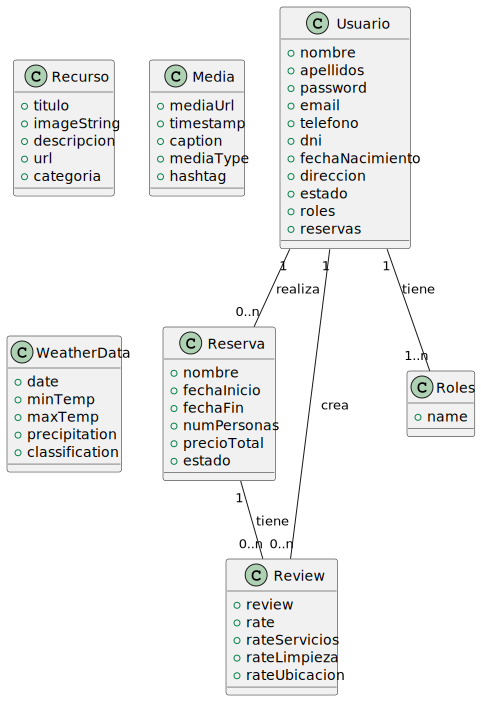
\includegraphics[width=1\textwidth]{figs/clases_simple.pdf}
    \caption{Diagrama general de clases.\label{fig:diagrama_clases}}
   
\end{figure}